\chapter*{ANEXE}
\addcontentsline{toc}{chapter}{ANEXE}
\markboth{ANEXE}{ANEXE}

\section*{Anexa 1: Capturi de Ecran}
\addcontentsline{toc}{section}{Anexa 1: Capturi de Ecran}
\markboth{Anexa 1: Capturi de Ecran}{Anexa 1: Capturi de Ecran}

\begin{figure}[h!]
    \centering
    \begin{minipage}{0.45\textwidth}
        \centering
        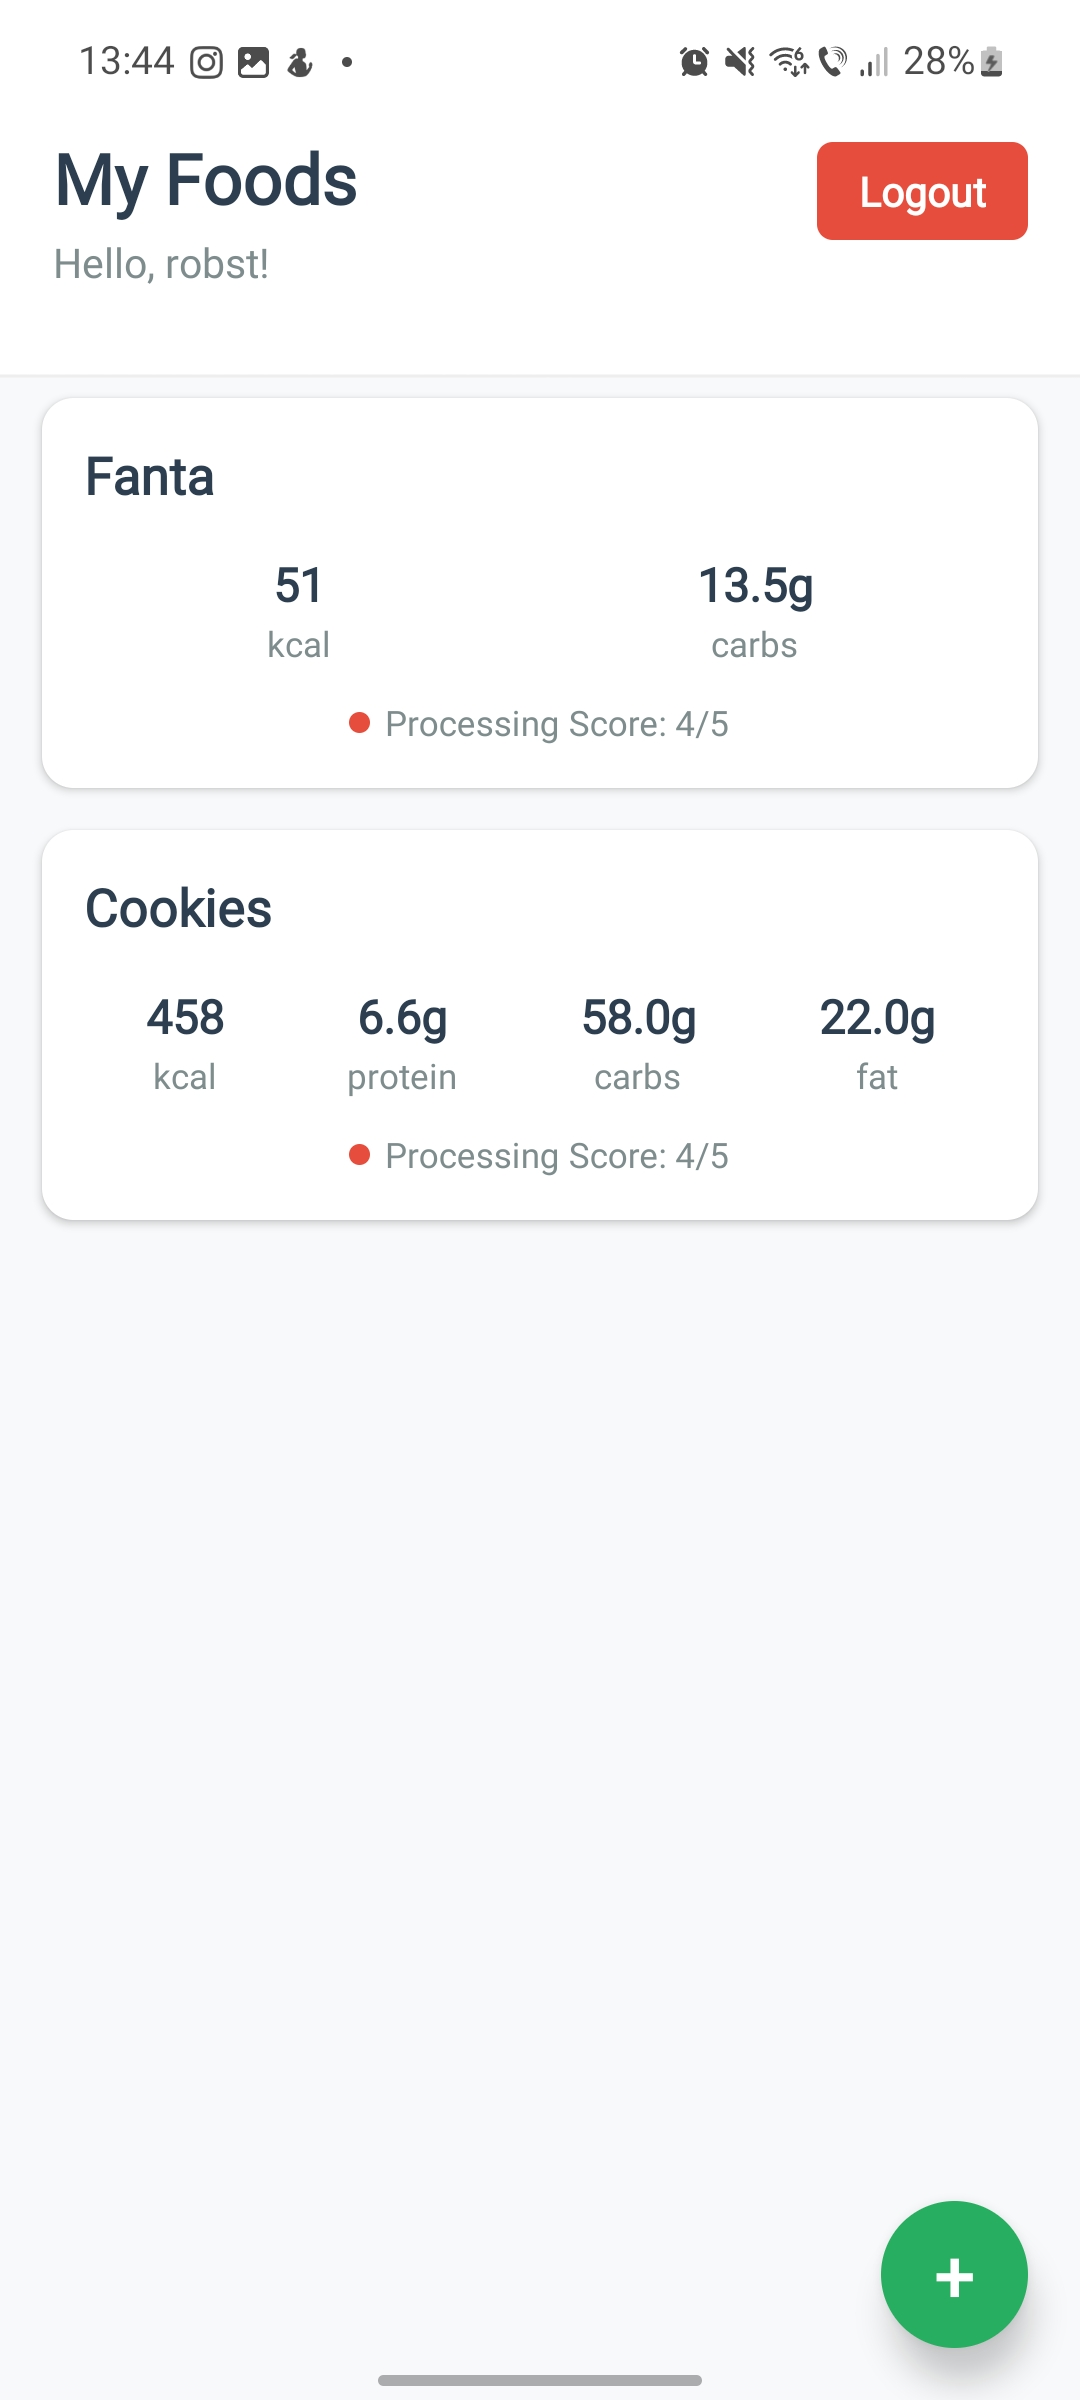
\includegraphics[width=0.9\textwidth]{images/Food_list.jpg}
        \caption{Lista de alimente adăugate de utilizator, afișând valorile nutriționale găsite și scorul de procesare.}
        \label{fig:food-list}
      \end{minipage}
    \hfill
    \begin{minipage}{0.45\textwidth}
        \centering
        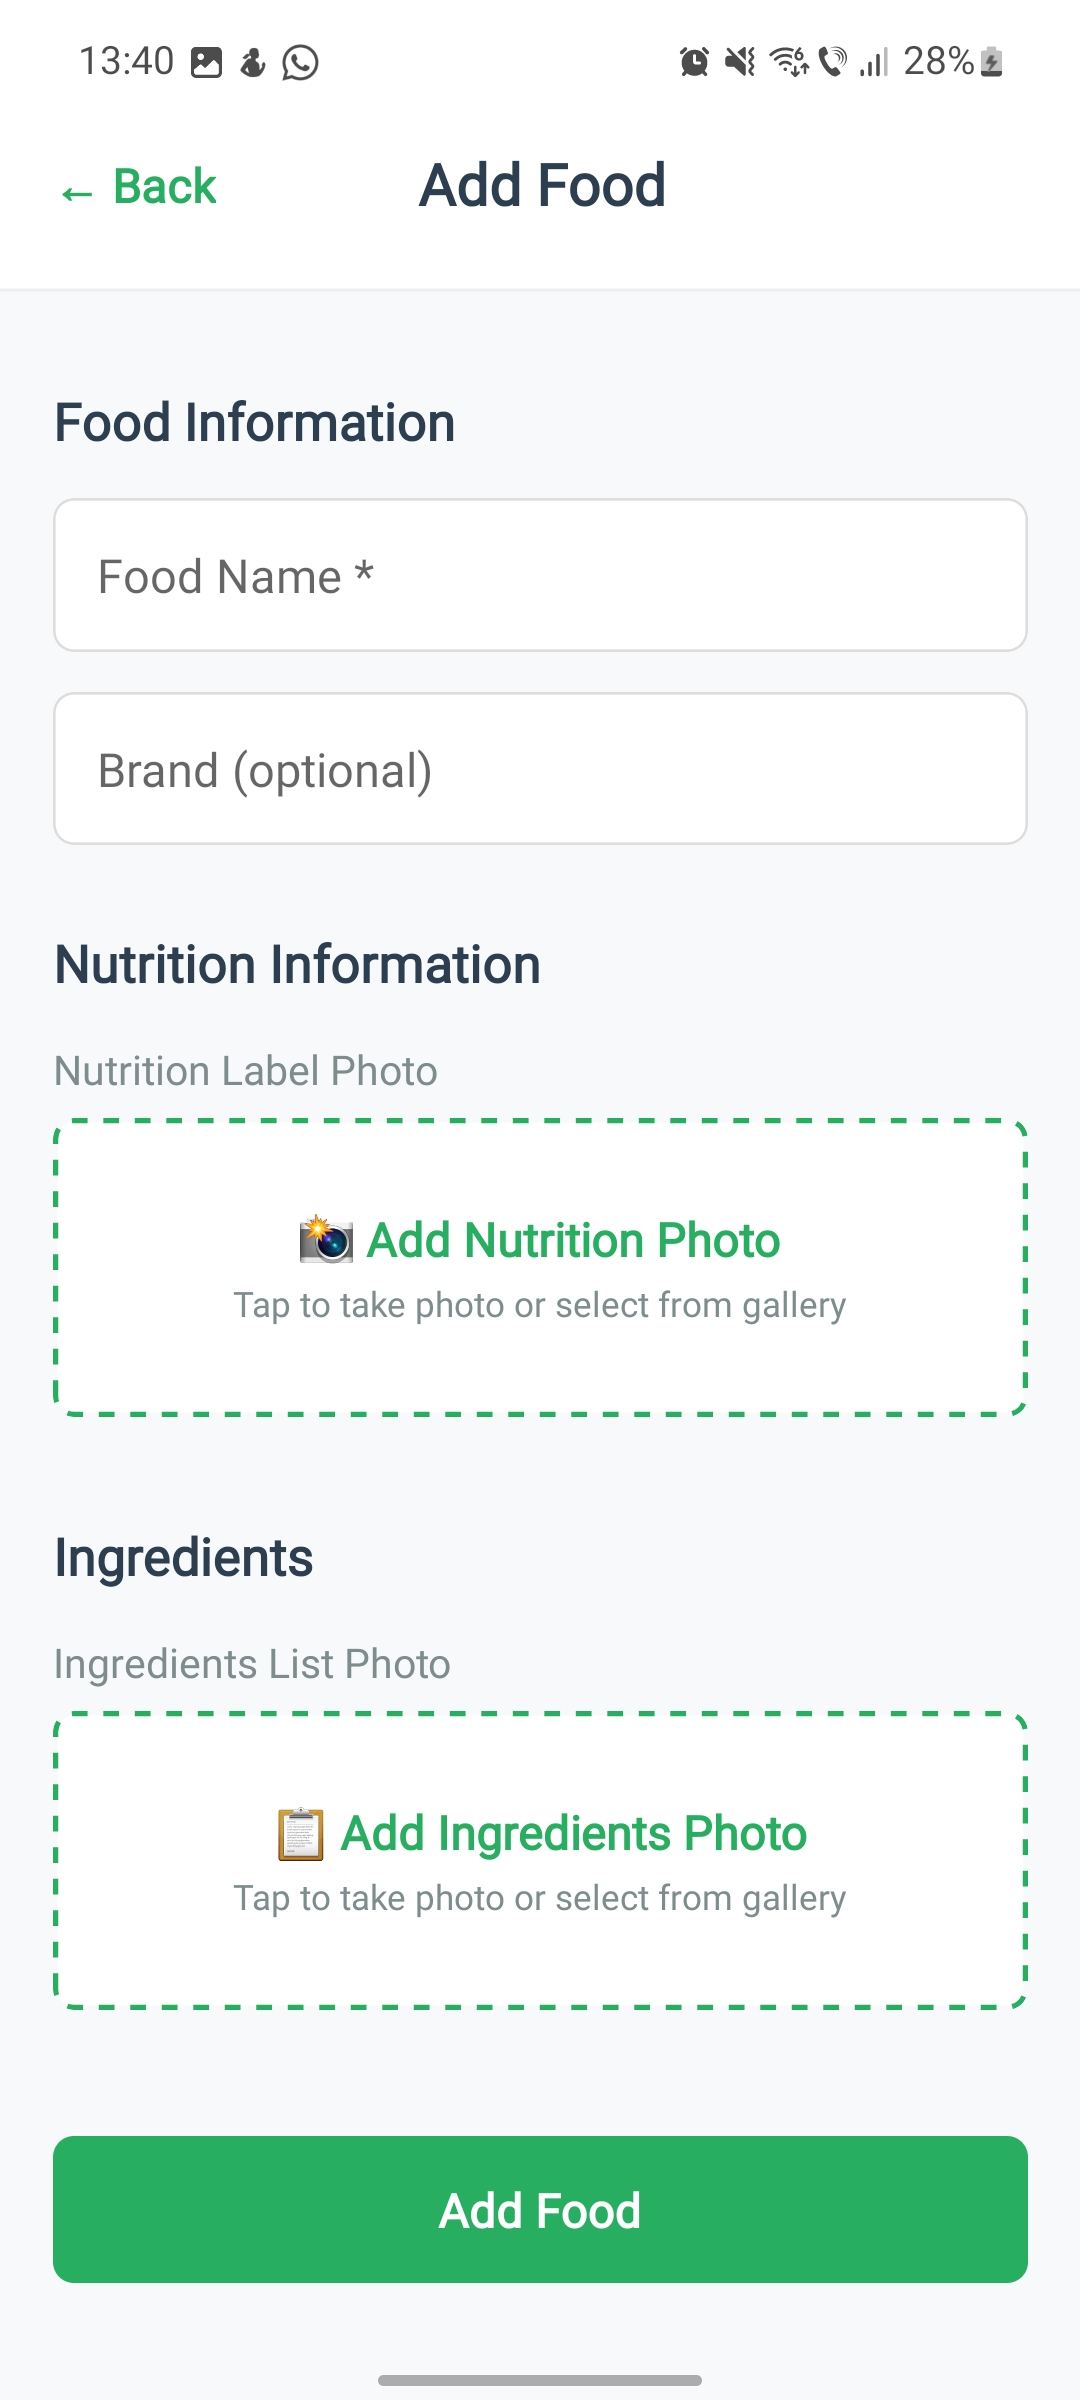
\includegraphics[width=0.9\textwidth]{images/Food_add.jpg}
        \caption{Ecranul de adăugare a unui nou aliment, unde utilizatorul poate încărca o poză cu eticheta alimentară.}
        \label{fig:food-add}
    \end{minipage}
\end{figure}

\begin{figure}[h!]
    \centering
    \begin{minipage}{0.45\textwidth}
        \centering
        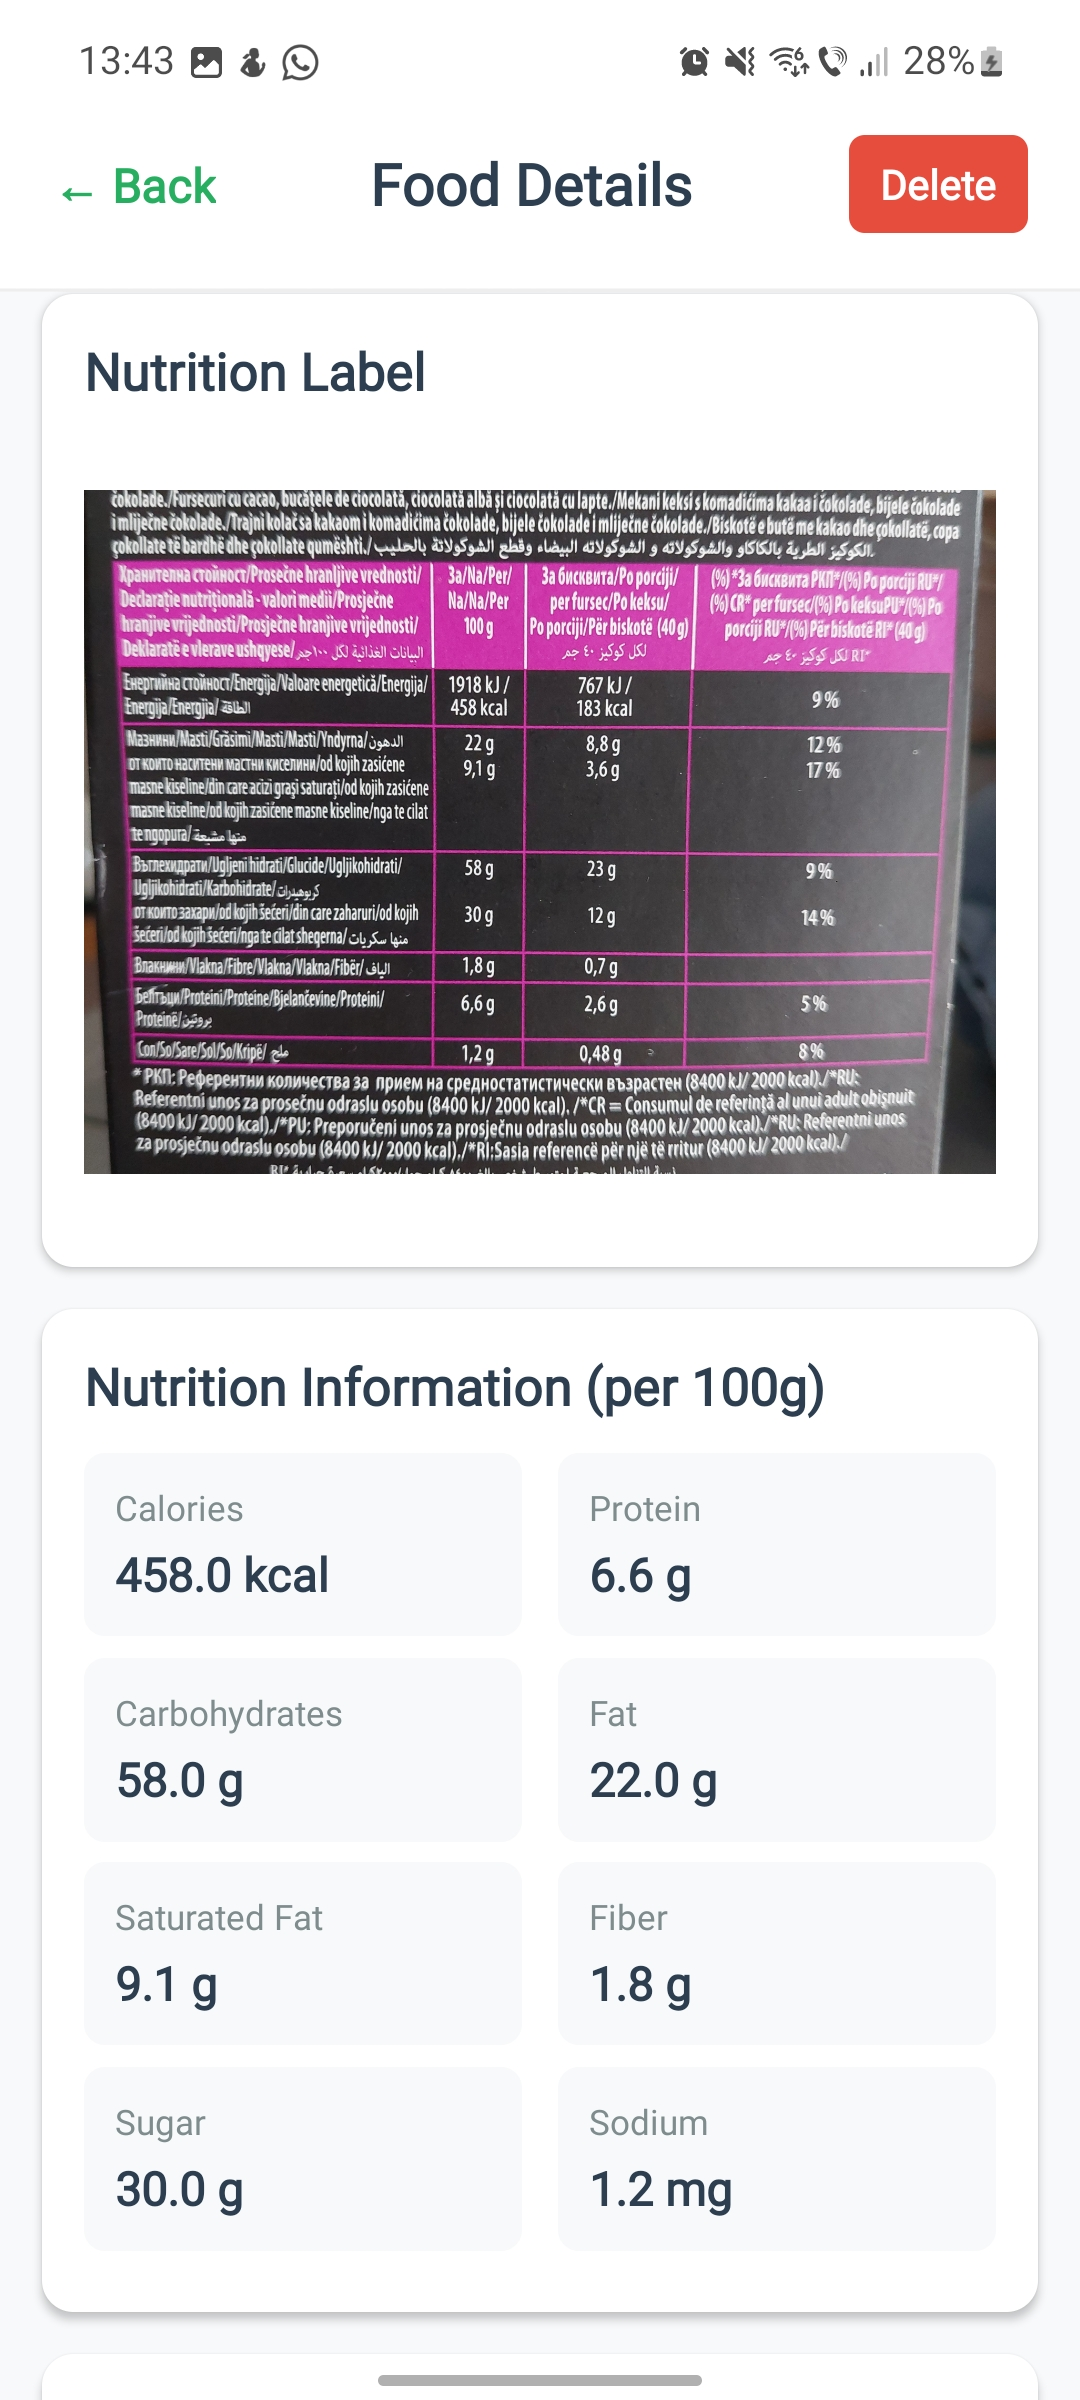
\includegraphics[width=0.9\textwidth]{images/Nutritional_info.jpg}
        \caption{Informațiile nutriționale extrase dintr-o etichetă alimentară.}
        \label{fig:nutritional-info}
    \end{minipage}
\end{figure}

\begin{figure}[h!]
    \centering
    \begin{minipage}{0.45\textwidth}
        \centering
        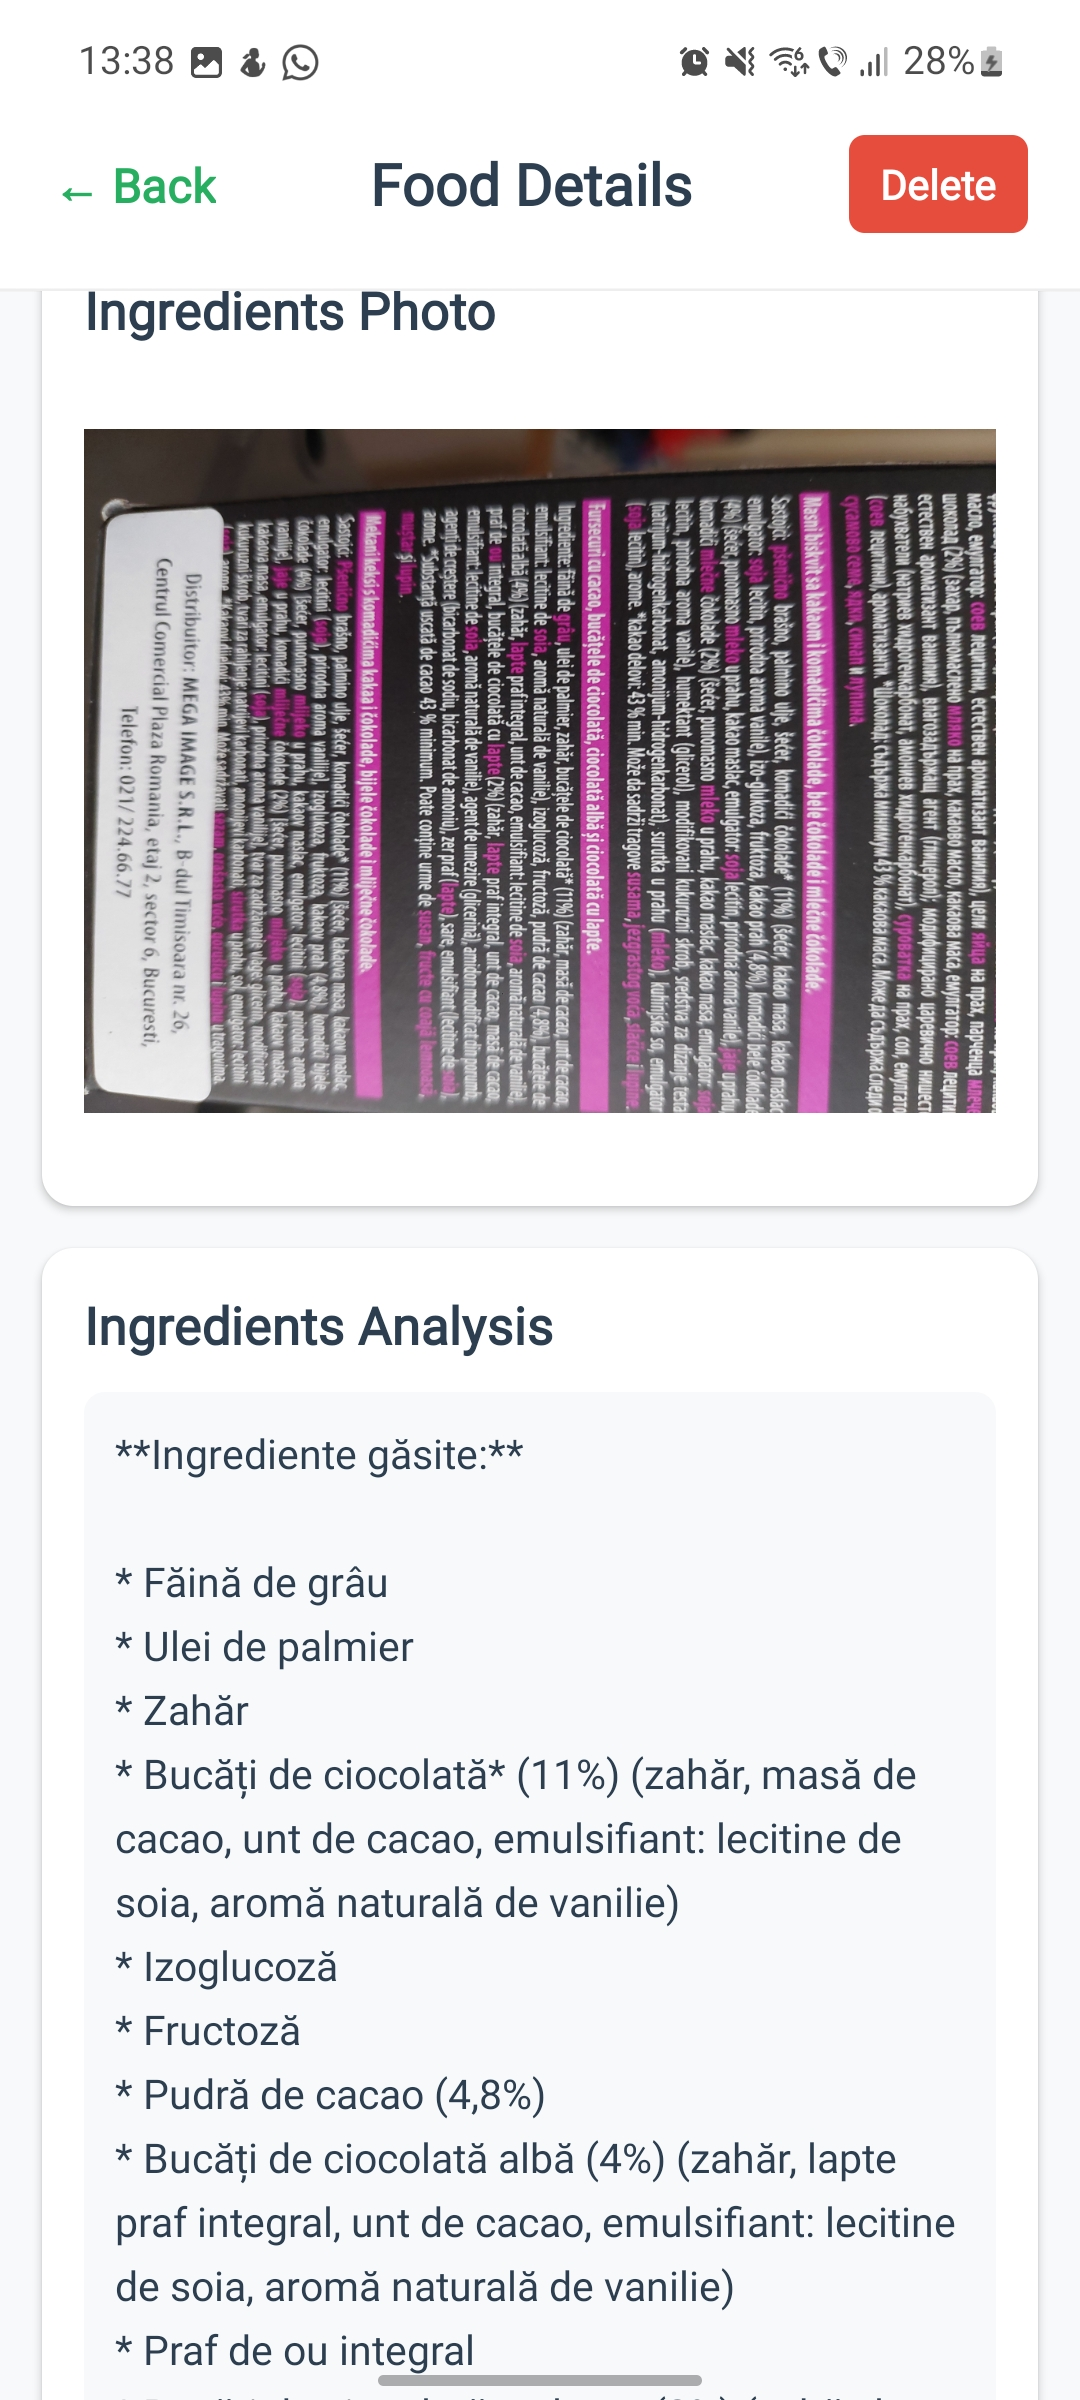
\includegraphics[width=0.9\textwidth]{images/Ingredients_info_1.jpg}
        \caption{Informațiile despre ingrediente extrase dintr-o poză cu ingrediente, afișând analiza detaliată generată de AI.}
        \label{fig:ingredients-info-1}
    \end{minipage}
    \hfill
    \begin{minipage}{0.45\textwidth}
        \centering
        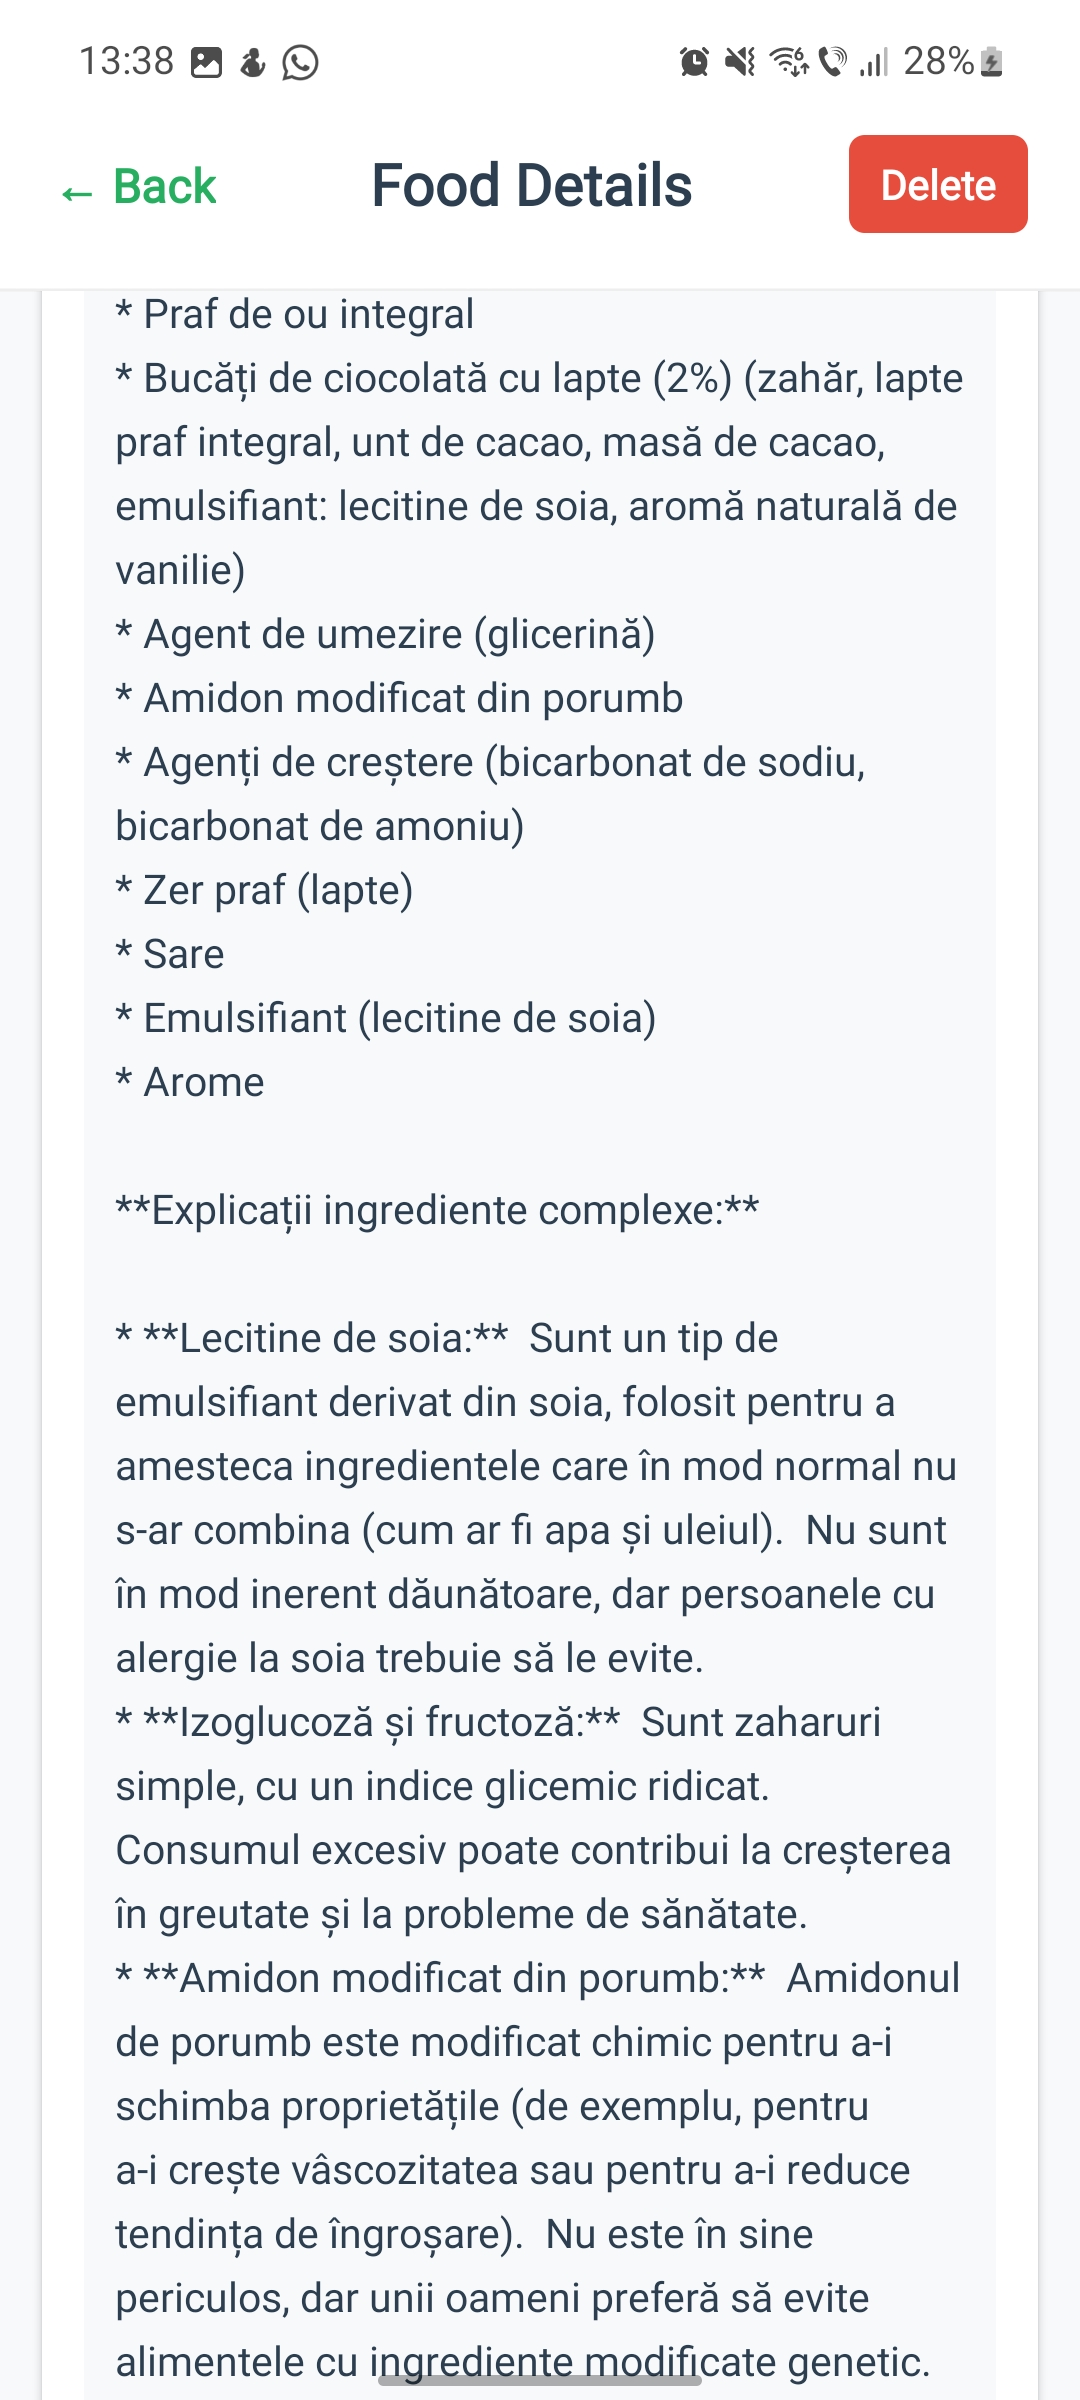
\includegraphics[width=0.9\textwidth]{images/Ingredients_info_2.jpg}
        \caption{Informațiile despre ingrediente extrase dintr-o poză cu ingrediente, evidențiind rolul fiecărui ingredient.}
        \label{fig:ingredients-info-2}
    \end{minipage}
\end{figure}

\begin{figure}[h!]
    \centering
    \begin{minipage}{0.45\textwidth}
        \centering
        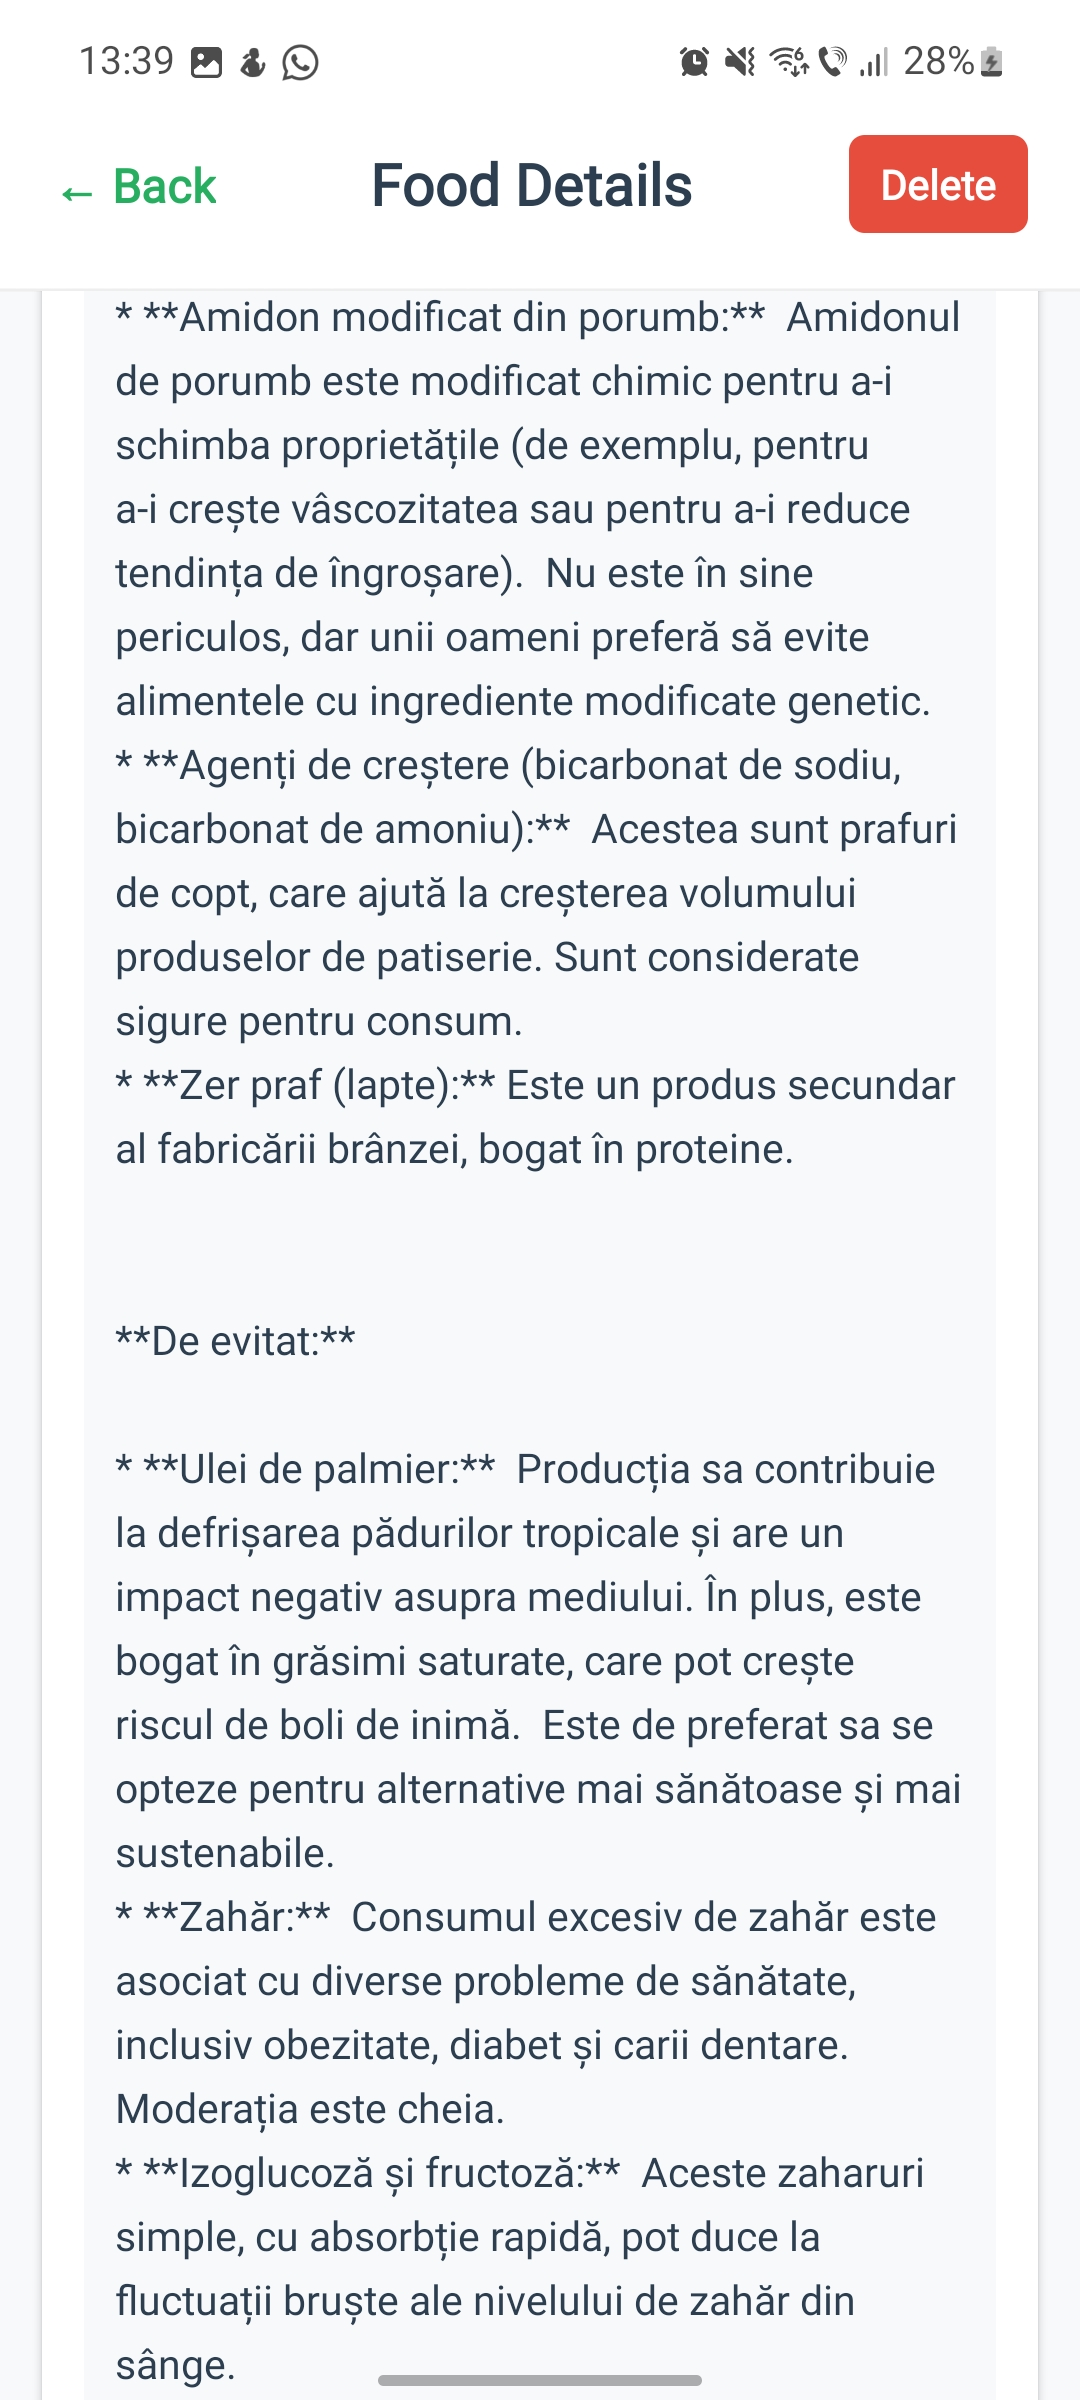
\includegraphics[width=0.9\textwidth]{images/Ingredients_info_3.jpg}
        \caption{Informațiile despre ingrediente extrase dintr-o poză cu ingrediente, afișând alimentele ce ar trebui evitate.}
        \label{fig:ingredients-info-3}
    \end{minipage}
    \hfill
    \begin{minipage}{0.45\textwidth}
        \centering
        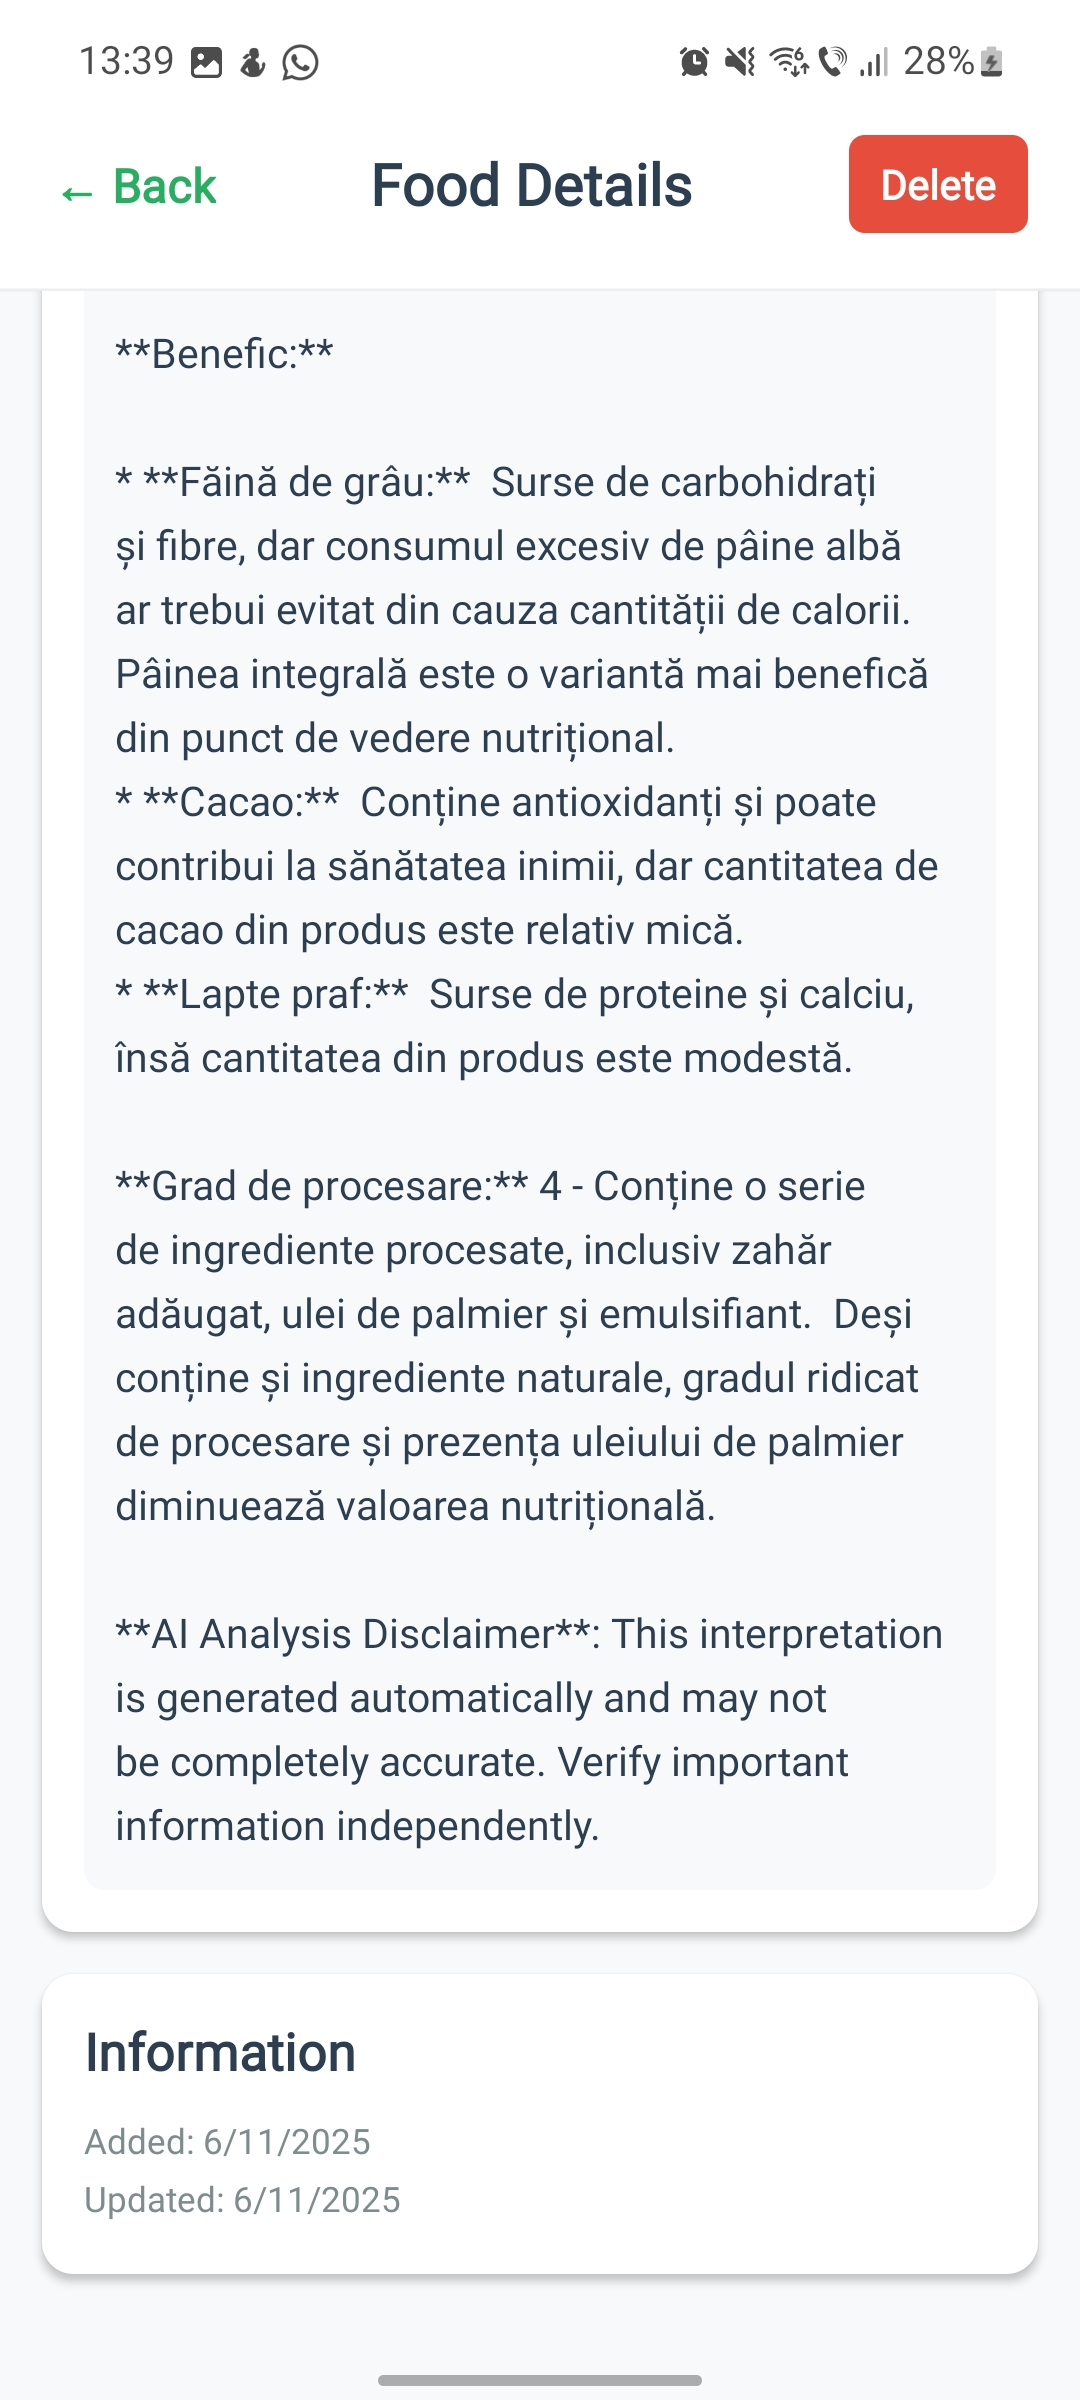
\includegraphics[width=0.9\textwidth]{images/Ingredients_info_4.jpg}
        \caption{Informațiile despre ingrediente extrase dintr-o poză cu ingrediente, evidențiind scorul de procesare și alimentele benefice.}
        \label{fig:ingredients-info-4}
    \end{minipage}
\end{figure}

\begin{figure}[h!]
    \centering
    \begin{minipage}{0.45\textwidth}
        \centering
        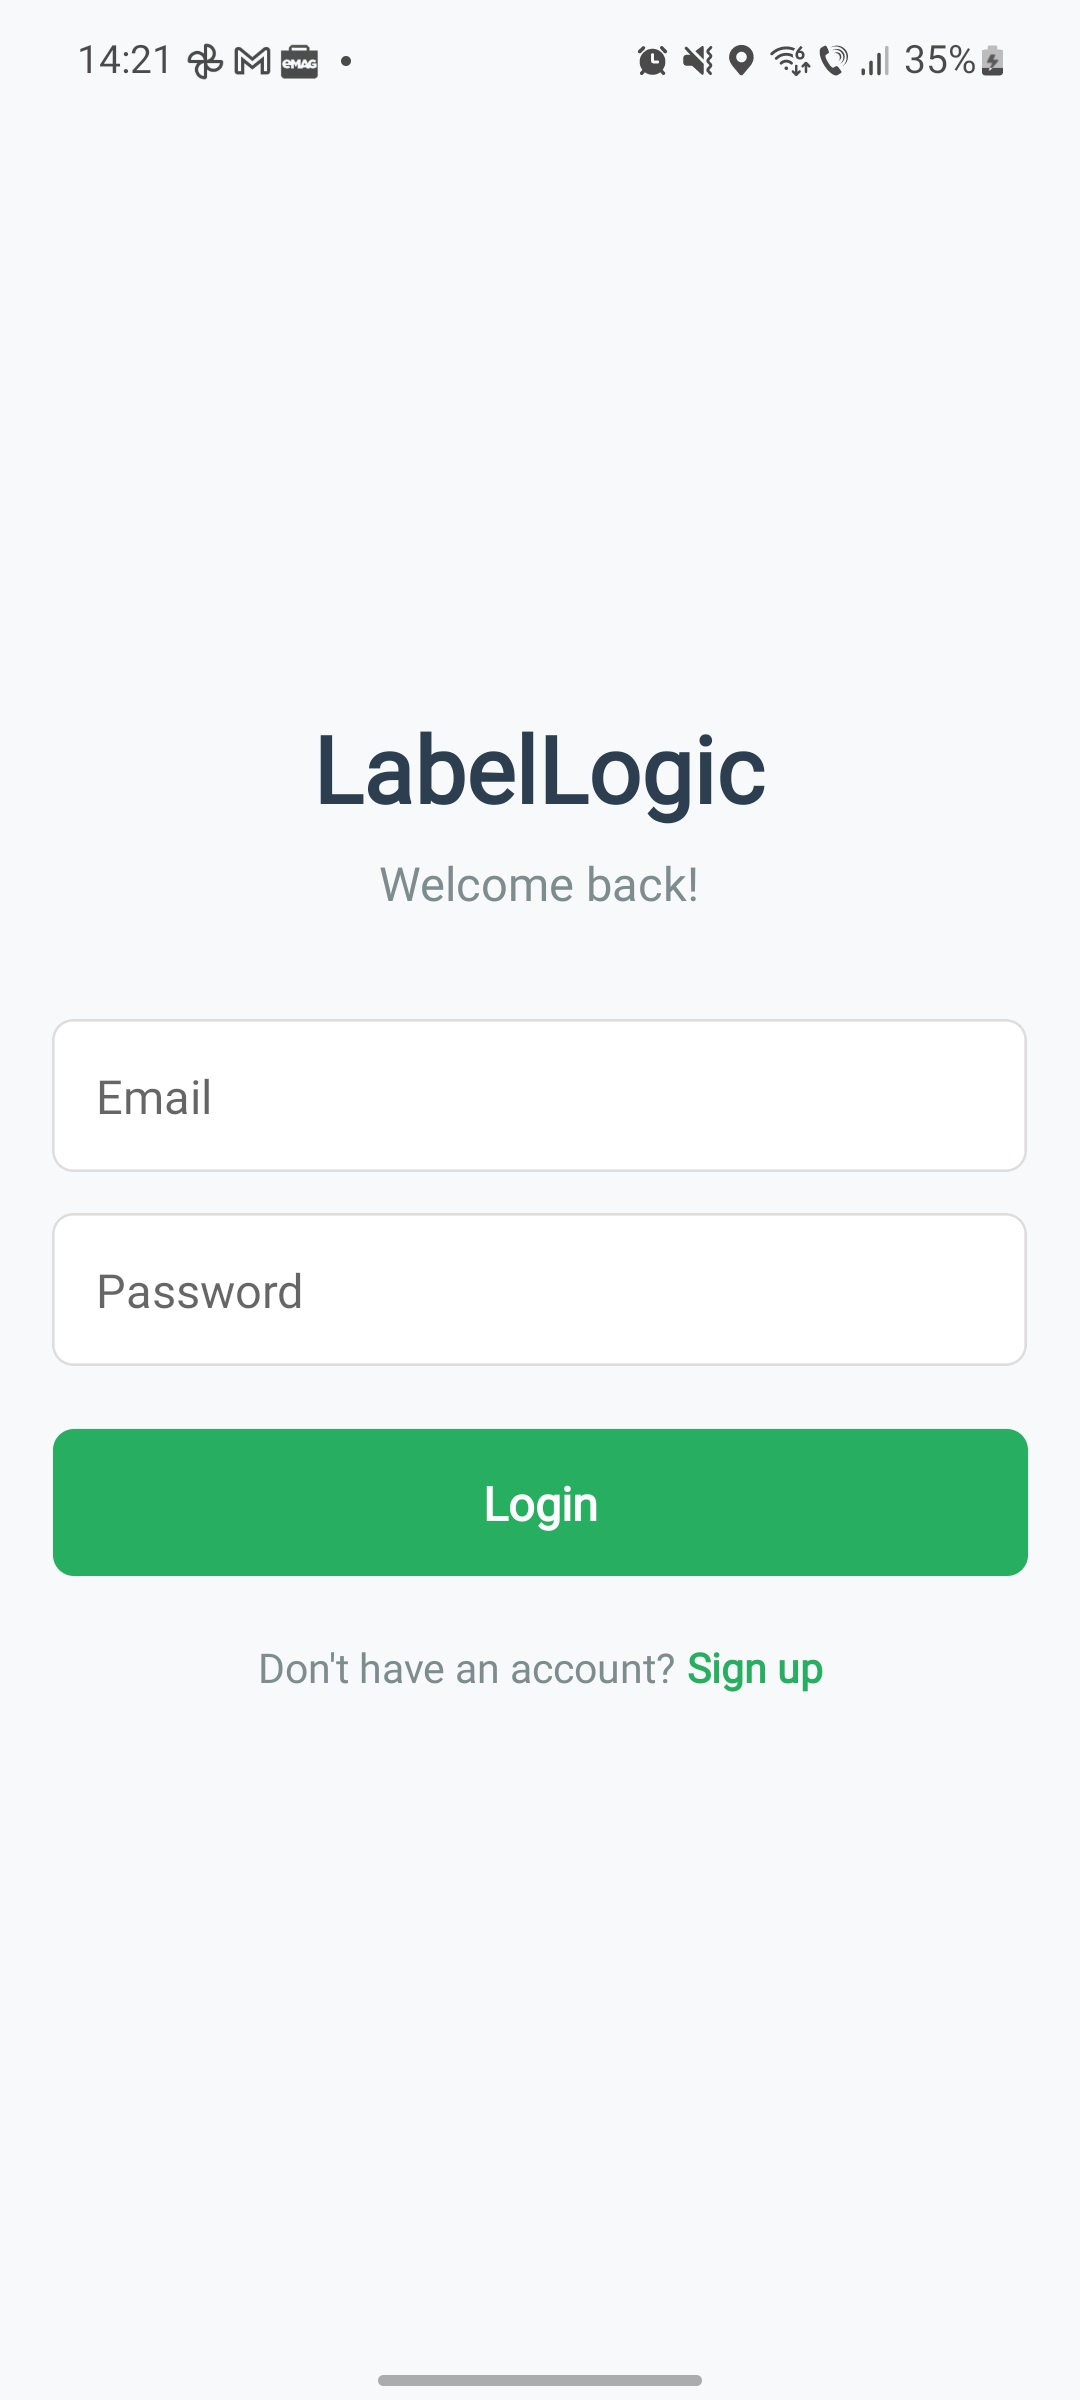
\includegraphics[width=0.9\textwidth]{images/Login.jpg}
        \caption{Pagina de autentificare a aplicației.}
        \label{fig:login}
    \end{minipage}
    \hfill
    \begin{minipage}{0.45\textwidth}
        \centering
        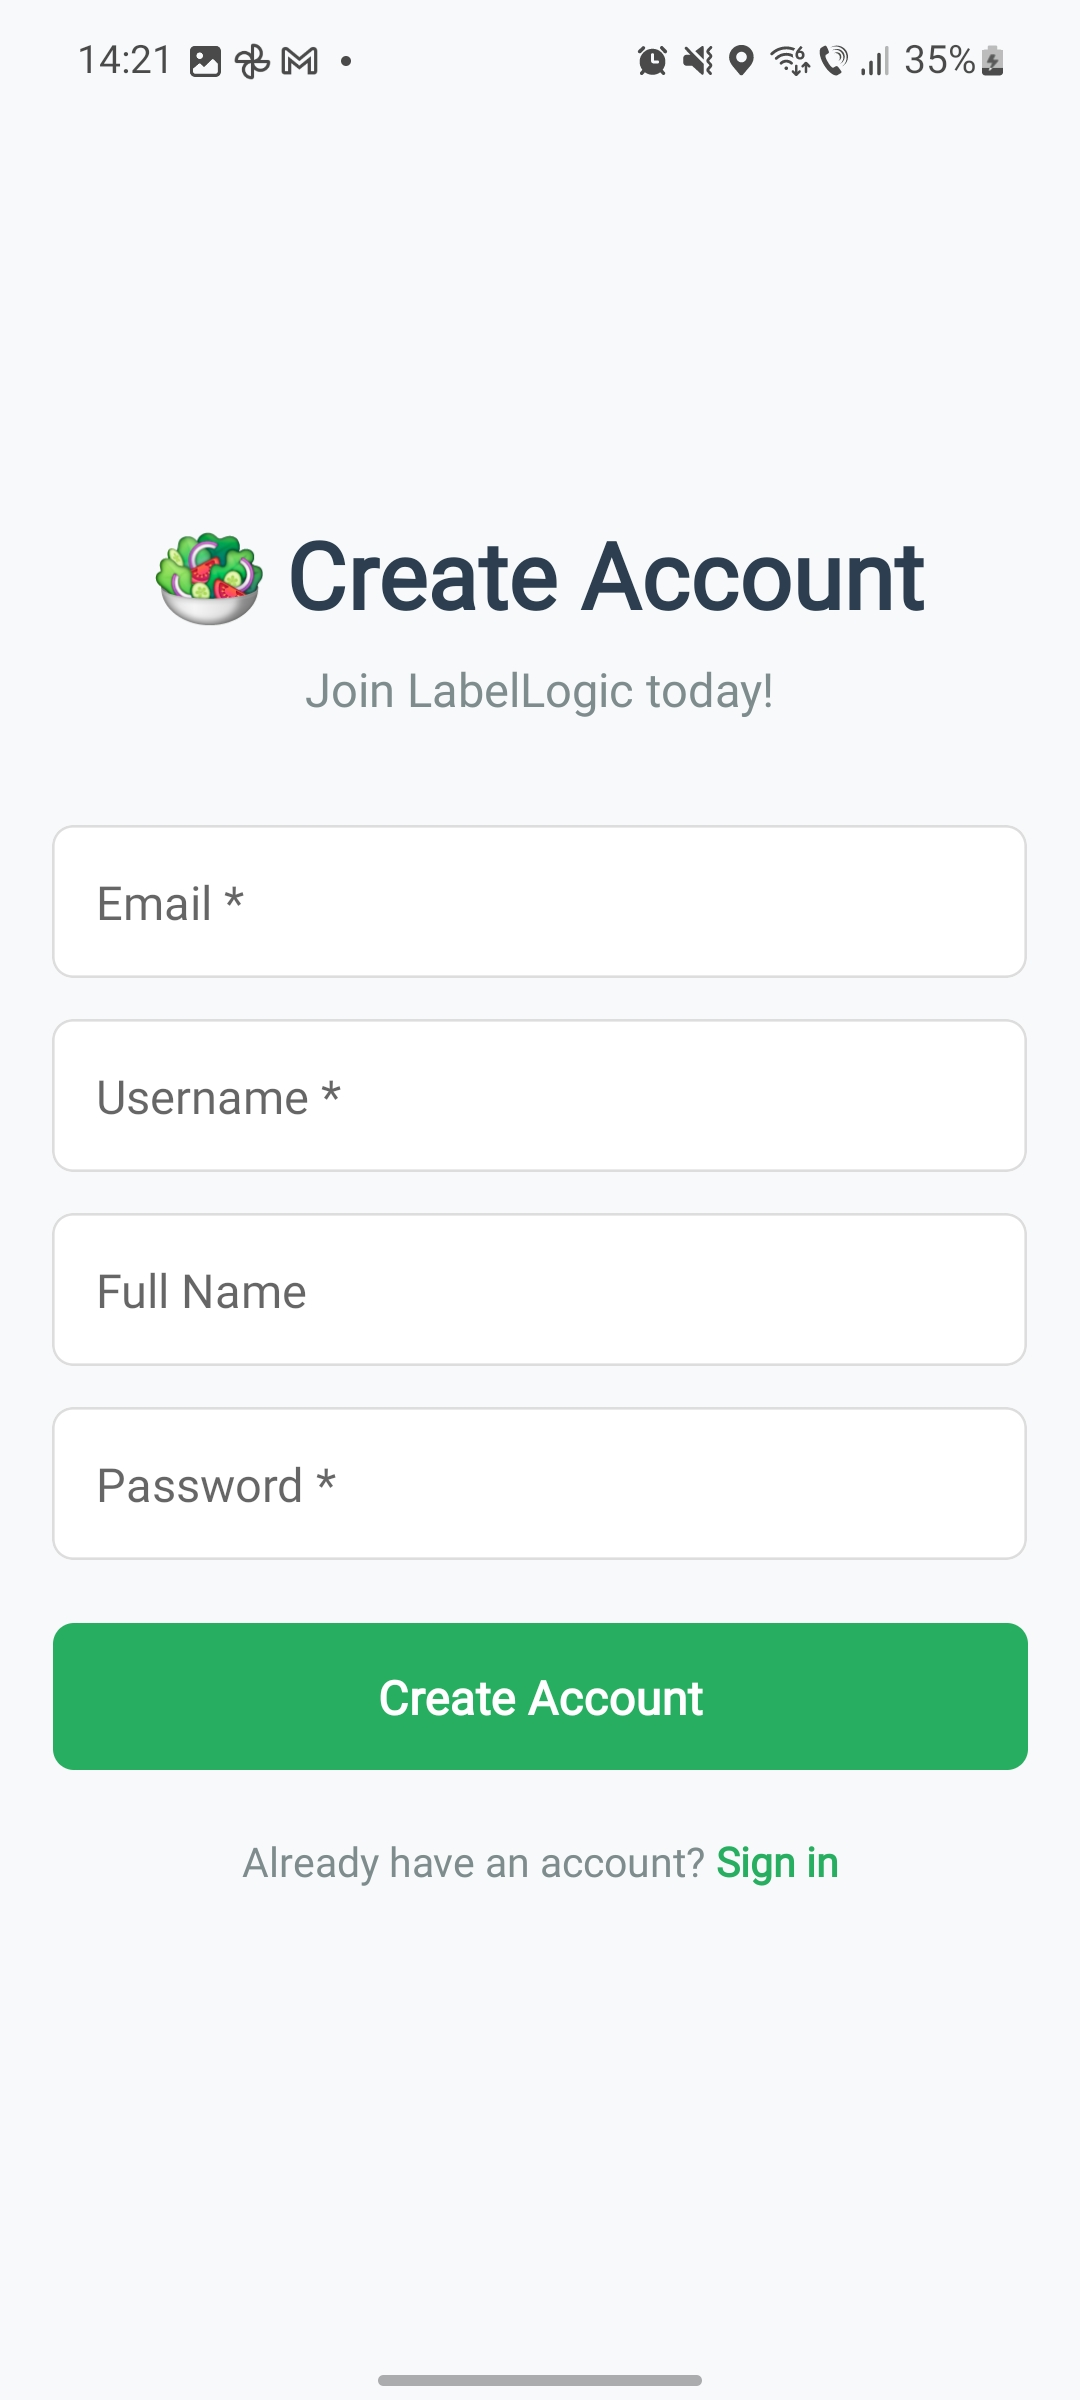
\includegraphics[width=0.9\textwidth]{images/Register.jpg}
        \caption{Pagina de înregistrare a aplicației.}
        \label{fig:register}
    \end{minipage}
\end{figure}